%%===========================================================%%
%%                                                           %%
%%                        CORRECTIONS                        %%
%%                                                           %%
%%===========================================================%%


\chapter{Corrections}\label{chap:corrections}

\section{Method of corrections application}
\begin{equation}
  \frac{d\sigma}{dq} = \frac{1}{\Delta q} \times \frac{1}{\varepsilon} \times \frac{N^{\mathit{w}}-N^{\mathit{w}}_\textrm{bkgd}}{\mathit{L}_{\textrm{int}}^{\textrm{eff}}}
\end{equation}

%remembed about accounting for RP trigger eff!!!
\begin{equation}\label{eq:effectiveLumi}
	\mathit{L}_{\textrm{int}}^{\textrm{eff}} = \sum\limits_{\textrm{run}}\mathit{L}_{\textrm{int}}^{\textrm{run}} \times \epsilon_{\textrm{veto}}(L^{\textrm{run}})
\end{equation}
% \left(\epsilon_{\textrm{veto}}^{\textrm{online}} \oplus \epsilon_{\textrm{veto}}^{\textrm{offline}}(L_{\textrm{run}}) \right)

\begin{equation}
	\varepsilon = \epsilon_{\textrm{\tiny ET/IT}} \times \epsilon_{\textrm{vrtx}}(q) \times \epsilon_{\ref{enum:CutZVx}} \times \epsilon_{\ref{enum:CutDeltaZVx}} \times \epsilon_{\ref{enum:CutMissingPt}} \times \epsilon_{\textrm{\tiny PID}}(q)
\end{equation}

\begin{equation}
	N^{\mathit{w}} = \sum\limits_{\textrm{event}}\mathit{w}_{\textrm{event}}
\end{equation}



\begin{equation}
	\mathit{w} = \left[\prod\limits_{\textrm{sign}} \epsilon_{\textrm{\tiny TOF}}(\textrm{sign}, \textrm{PID}, p_{T},z_{vx},\eta)  \times \prod\limits_{\textrm{sign}} \epsilon_{\textrm{\tiny TPC}}(\textrm{sign}, \textrm{PID}, p_{T},z_{vx},\eta) \times \prod\limits_{\textrm{side}}\epsilon_{\textrm{\tiny RP}}^{\textrm{side}}(p_{x},p_{y}) \right]^{-1},
\end{equation}
\[\textrm{sign}=\{+,-\},~~\textrm{side}=\{E,W\}\]
% ()

\section{Efficiencies and acceptances}
\subsection{Trigger efficiency}\label{sec:triggerEff}
\subsubsection{Online veto (BBC-small and ZDC veto)}
%---------------------------
\begin{figure}[ht!]
\centering%
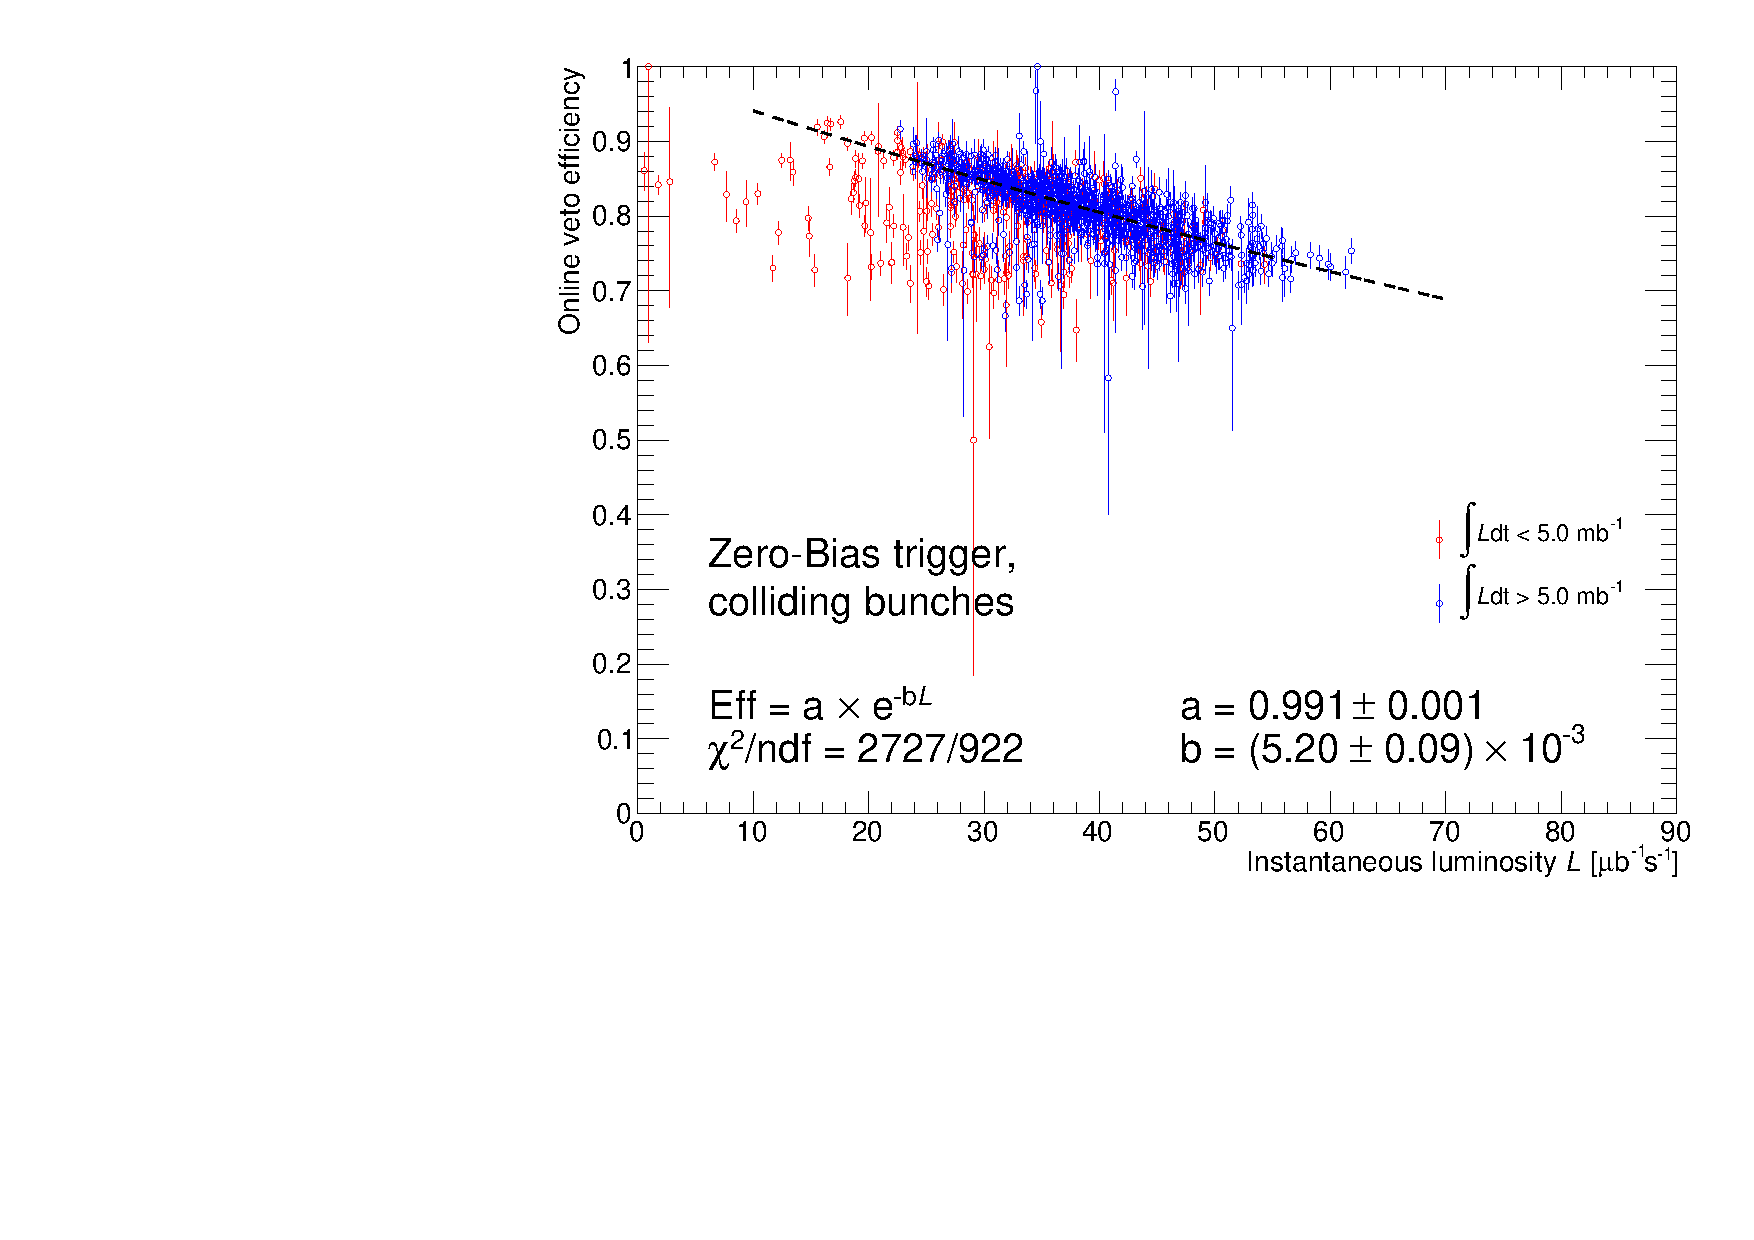
\includegraphics[width=0.65\linewidth,page=1]{graphics/corrections/OnlineVetoEffVsInstLumi_graph.pdf}%
\caption{Overall efficiency of the online BBC-small and ZDC veto as a function of instantaneous luminosity.}\label{fig:onlineVetoEff}%
\end{figure}
%---------------------------
\subsubsection{RP triggering efficiency}
\subsubsection{Up and Down RP combination veto}
\subsection{Cuts efficiency}\label{sec:cutsEff}
\subsubsection{TPC \texorpdfstring{$z$}{z}-vertex cut~(\ref{enum:CutZVx})}
\subsubsection{TPC-RP \texorpdfstring{$z$}{z}-vertex matching~(\ref{enum:CutDeltaZVx})}
\subsubsection{Primary vertices limit~(\ref{enum:CutPrimVx}), BBC-large veto~(\ref{enum:CutBbcLarge}) and TOF clusters limit~(\ref{enum:CutTofClusters})}
%---------------------------
\begin{figure}[ht!]
\centering%
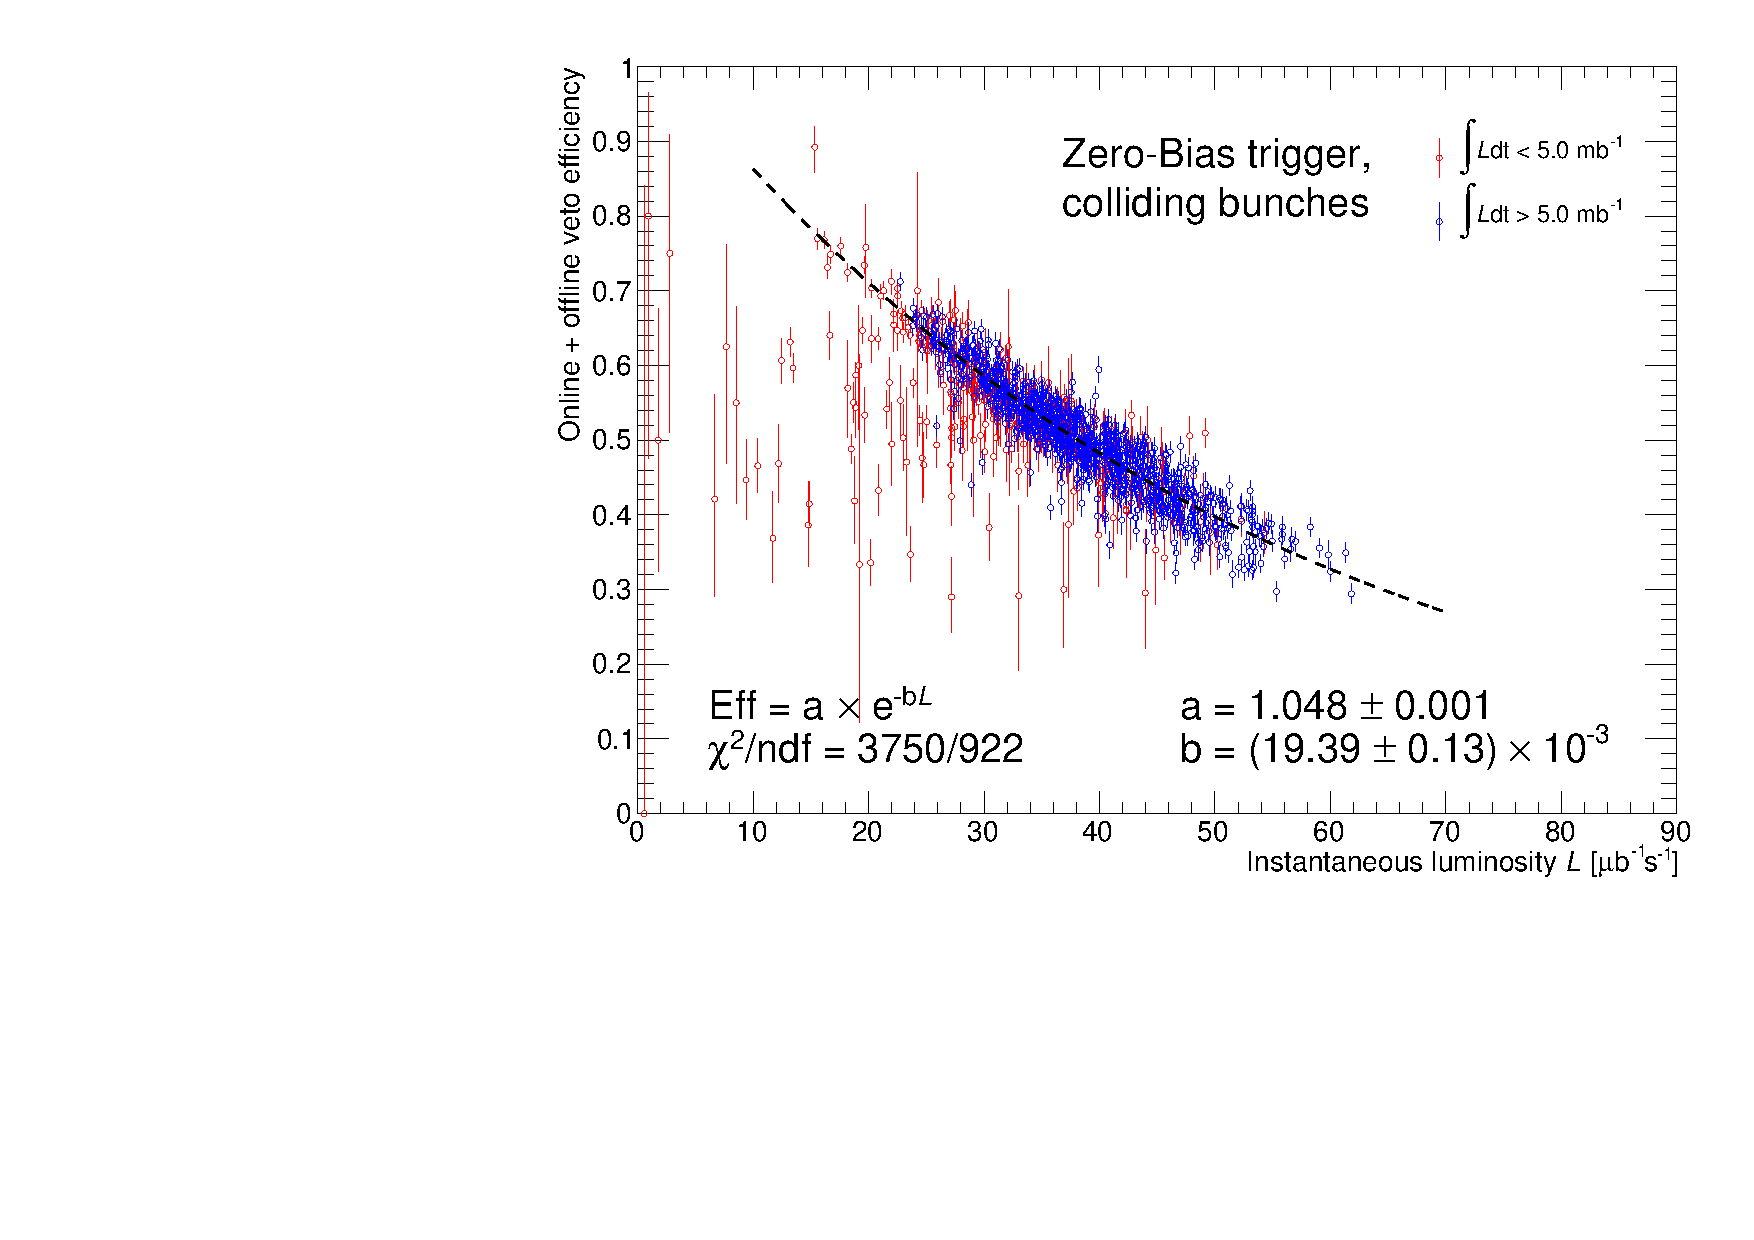
\includegraphics[width=0.65\linewidth,page=1]{graphics/corrections/OnlineAndOfflineVetoEffVsInstLumi_graph.pdf}%
\caption{Overall efficiency of the online BBC-small and ZDC veto, primary vertices limit~(\ref{enum:CutPrimVx}), BBC-large veto~(\ref{enum:CutBbcLarge}) and TOF clusters limit~(\ref{enum:CutTofClusters}) as a function of instantaneous luminosity.}\label{fig:onlineAndOfflineVetoEff}%
\end{figure}
%---------------------------
\subsubsection{Missing \texorpdfstring{$p_{T}$}{pT} cut~(\ref{enum:CutMissingPt})}
\subsubsection{Particle identification~(\ref{enum:CutPid})}

It is possible to transform dE/dx in MC to make it follow the shape of dE/dx in the data. 
We know that nSigmaX (where X=Pion, Kaon, Proton, ...) variable follows a gaussian distribution (for particle X)
 \[nSigmaX = \Big( \ln{\frac{dE/dx}{\langle dE/dx\rangle_{X}}} \Big) / \sigma_{dE/dx},~~~~~f(nSigmaX) = \mathcal{N}(nSigmaX; \mu=0,\sigma=1)\]
therefore $dE/dx$ itself follows log-normal distribution:
\[f(dE/dx) = \mathcal{L}og\mathcal{N}(dE/dx; \mu=\langle dE/dx\rangle,\sigma=\sigma_{dE/dx}) = \frac{1}{\sqrt{2\pi}\cdot \sigma\cdot dE/dx}e^{-\frac{\ln^{2}{\frac{dE/dx}{\langle dE/dx\rangle}}}{2\sigma^{2}}}\]
The transformation we want to apply should preserve the shape of $dE/dx$ (so that it is still described by $\mathcal{L}og\mathcal{N}$), however it should change $\mu$ and $\sigma$ so that these values are euqal to those seen in the data. The transformation that satisfies above postulate is
\[dE/dx' = c\cdot (dE/dx)^{a}\]
Parameters of the distribution $\mathcal{L}og\mathcal{N}(dE/dx')$ would be then
\[\mu' = c\cdot\mu^{a},~~~~\sigma' = a\cdot\sigma\]
From above we get formulae for parameters of the transformation:
\[a=\sigma'/\sigma,~~~~c = \frac{\mu'}{\mu^{a}}\]

AlternativeToCrystallBall~\cite{AlternativeToCrystallBall}~Eq.~\eqref{eq:expTail}

\begin{equation}\label{eq:expTail}
	f(dE/dx)=\left\{
                \begin{array}{ll}
                  \frac{A}{\sqrt{2\pi}\cdot \sigma\cdot dE/dx}\exp{\Bigg(-\frac{1}{2}\Big(\frac{\ln{\frac{dE/dx}{\langle dE/dx\rangle}}}{\sigma}\Big)^{2}\Bigg)} & \textrm{for}~\frac{\ln{\frac{dE/dx}{\langle dE/dx\rangle}}}{\sigma} \leq k \\
                  \frac{A}{\sqrt{2\pi}\cdot \sigma\cdot dE/dx}\exp{\Bigg(-k\cdot \frac{\ln{\frac{dE/dx}{\langle dE/dx\rangle}}}{\sigma} + \frac{1}{2}k^{2} - k^{-1}\left(\frac{\frac{\ln{\frac{dE/dx}{\langle dE/dx\rangle}}}{\sigma}}{k}-1\right)^{k} \Bigg)} & \textrm{for}~\frac{\ln{\frac{dE/dx}{\langle dE/dx\rangle}}}{\sigma} > k
                \end{array}
              \right.
\end{equation}


%---------------------------
\begin{figure}[hb]
\centering
\parbox{0.4725\textwidth}{
  \centering
  \begin{subfigure}[b]{\linewidth}{
                \subcaptionbox{\label{fig:dEdxMeanOffsetMC}}{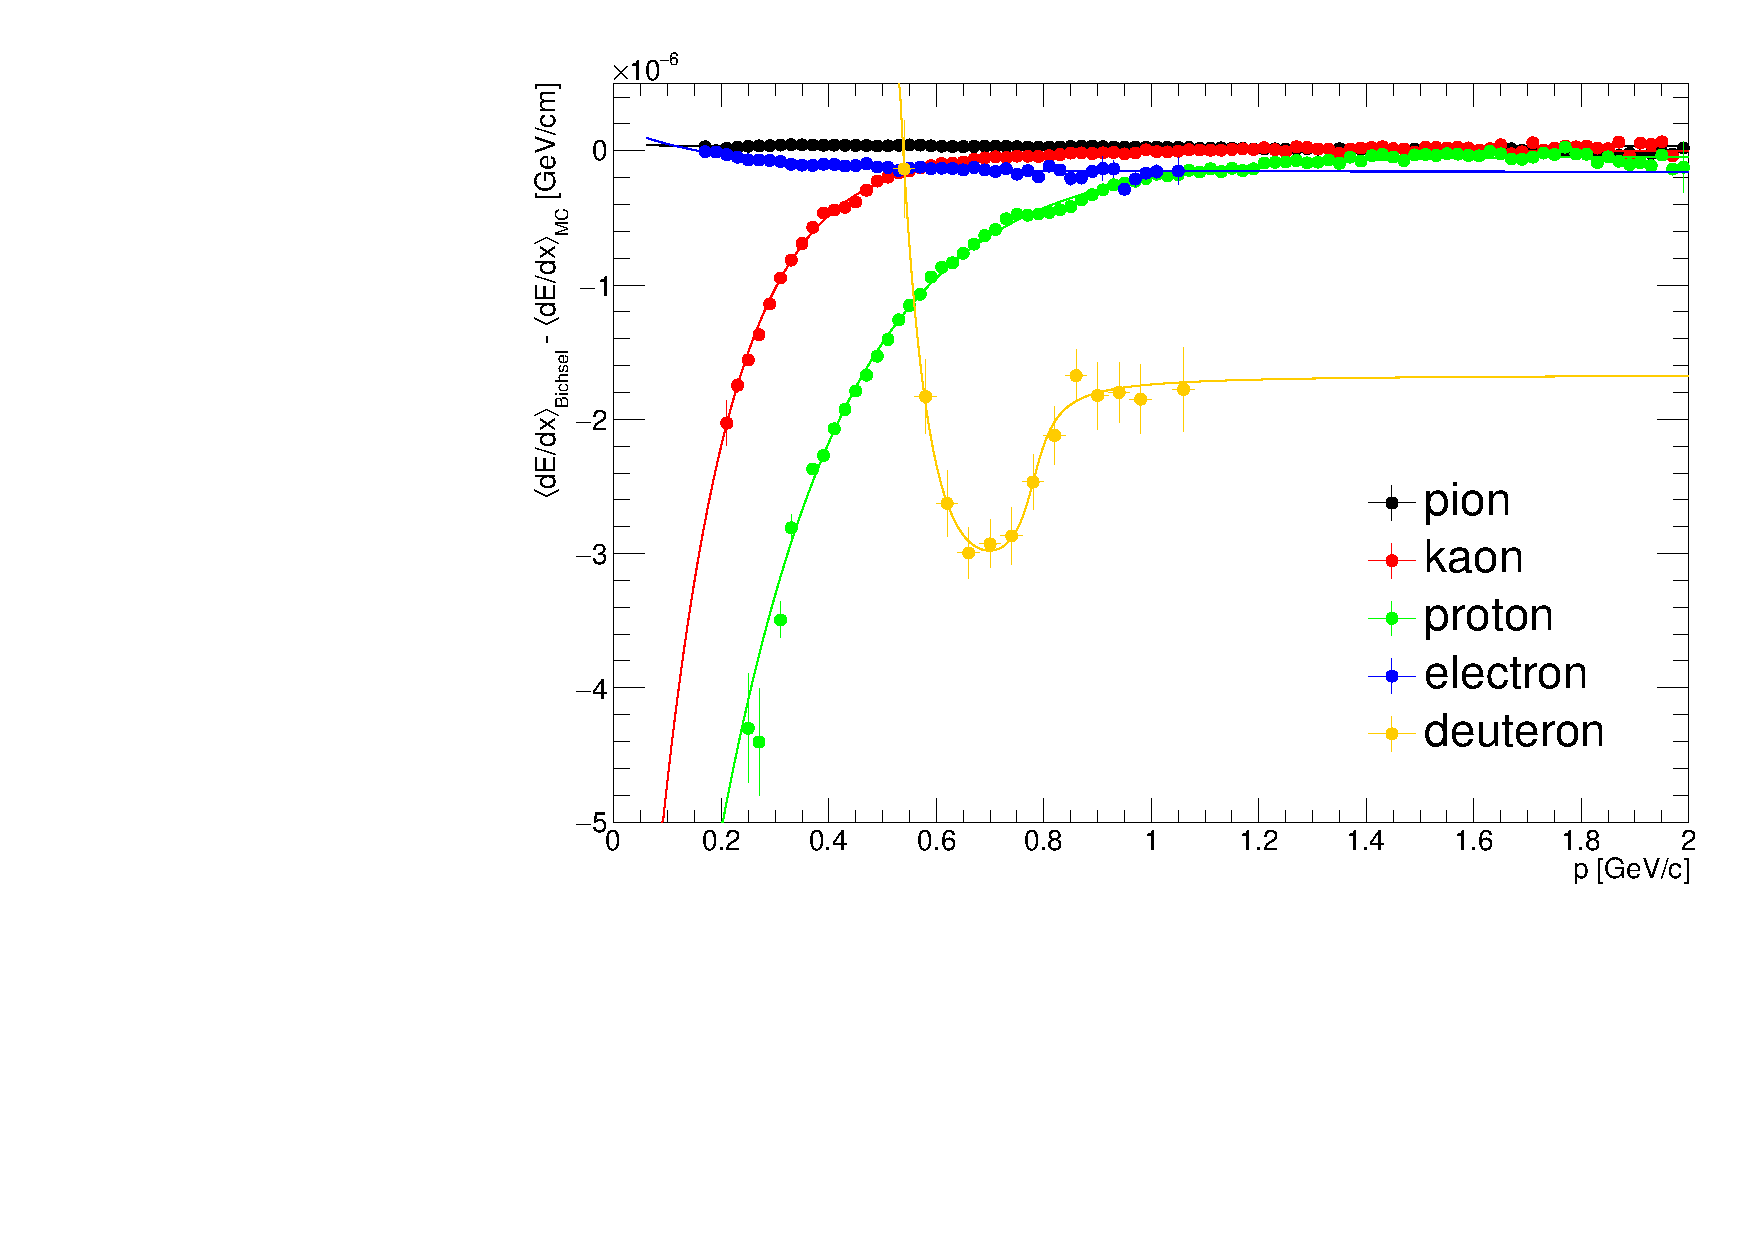
\includegraphics[width=\linewidth]{graphics/corrections/dEdxMeanOffset_allPIDs.pdf}\vspace*{-10pt}}}
  \end{subfigure}\\
  \begin{subfigure}[b]{\linewidth}\addtocounter{subfigure}{1}{
                \subcaptionbox{\label{fig:dEdxMeanOffsetData}}{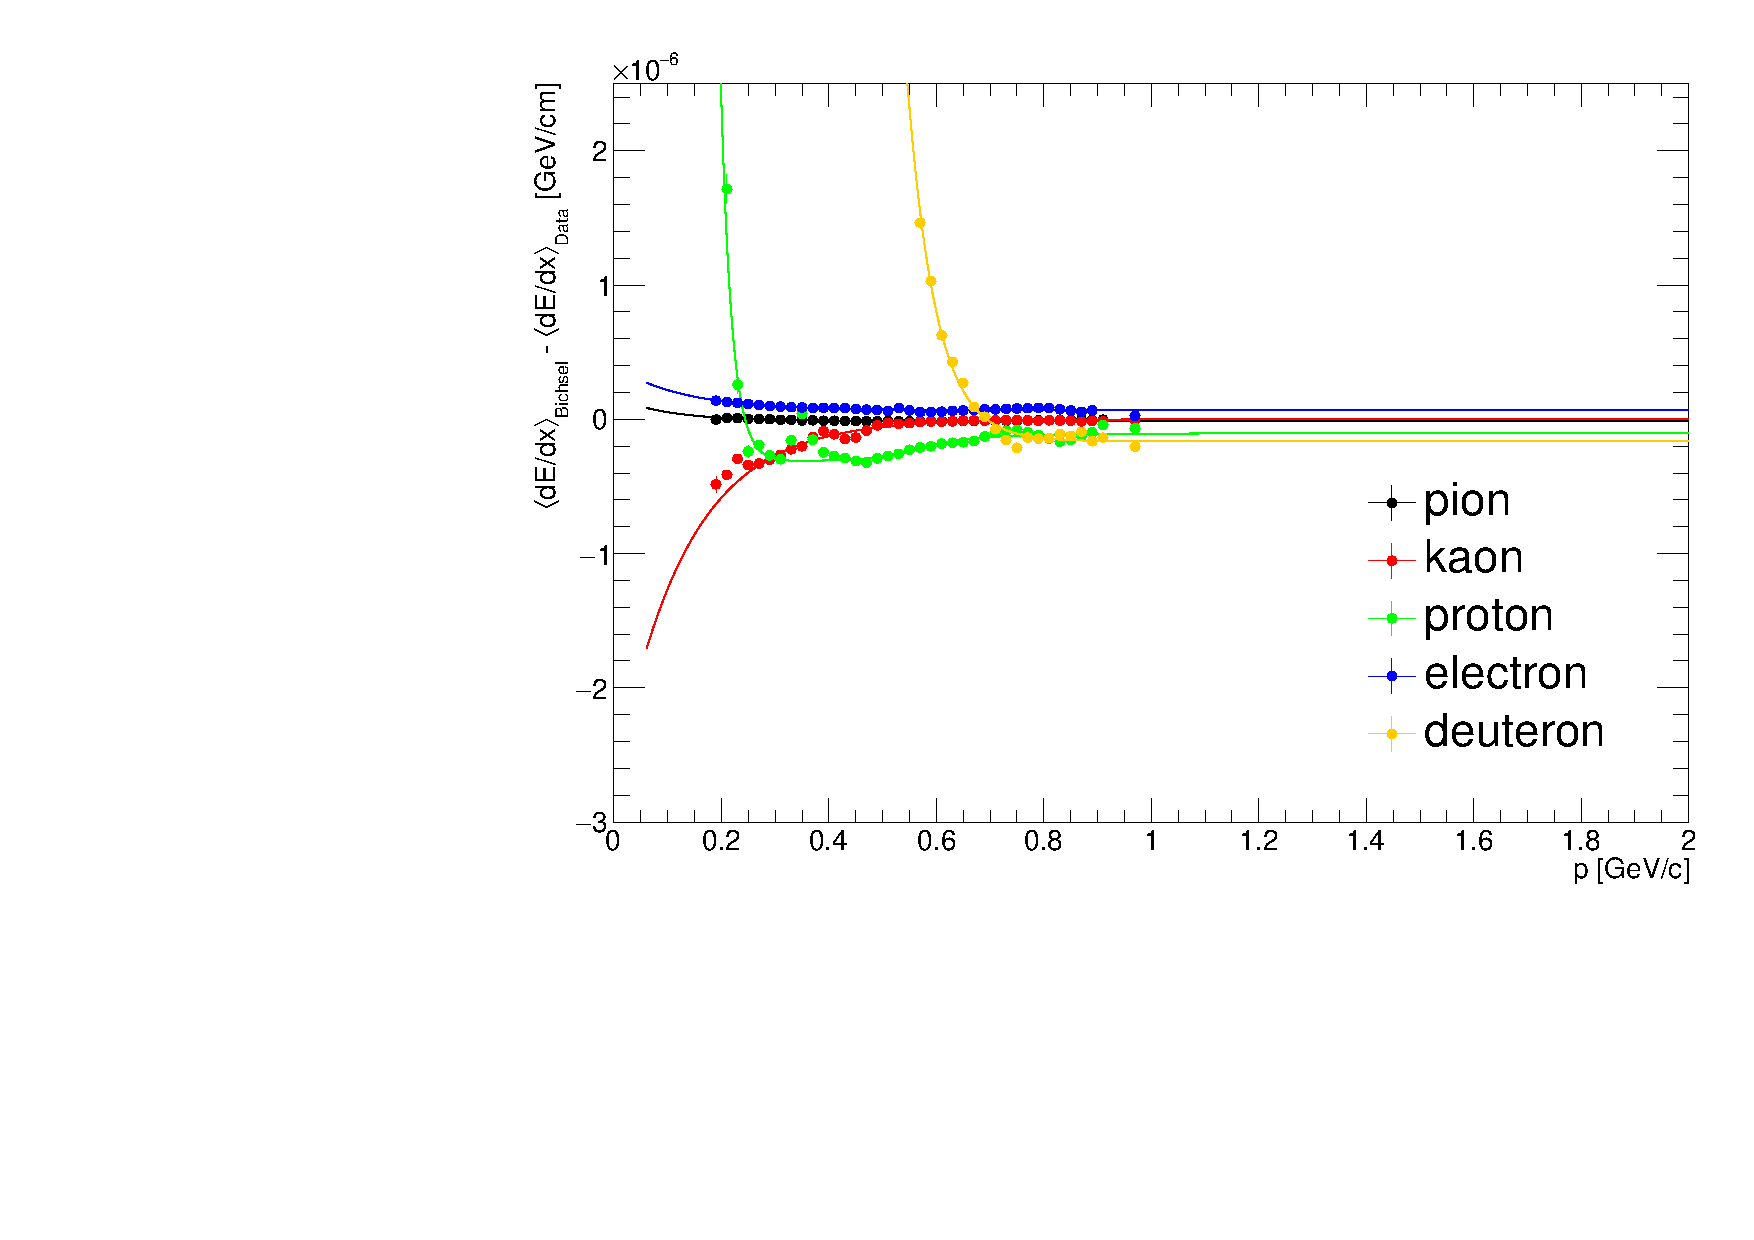
\includegraphics[width=\linewidth]{graphics/corrections/dEdxMeanOffset_allPIDs_data.pdf}\vspace*{-10pt}}}
  \end{subfigure}
}
\quad
\parbox{0.4725\textwidth}{
  \centering
  \begin{subfigure}[b]{\linewidth}\addtocounter{subfigure}{-2}{
                \subcaptionbox{\label{fig:dEdxWidthMC}}{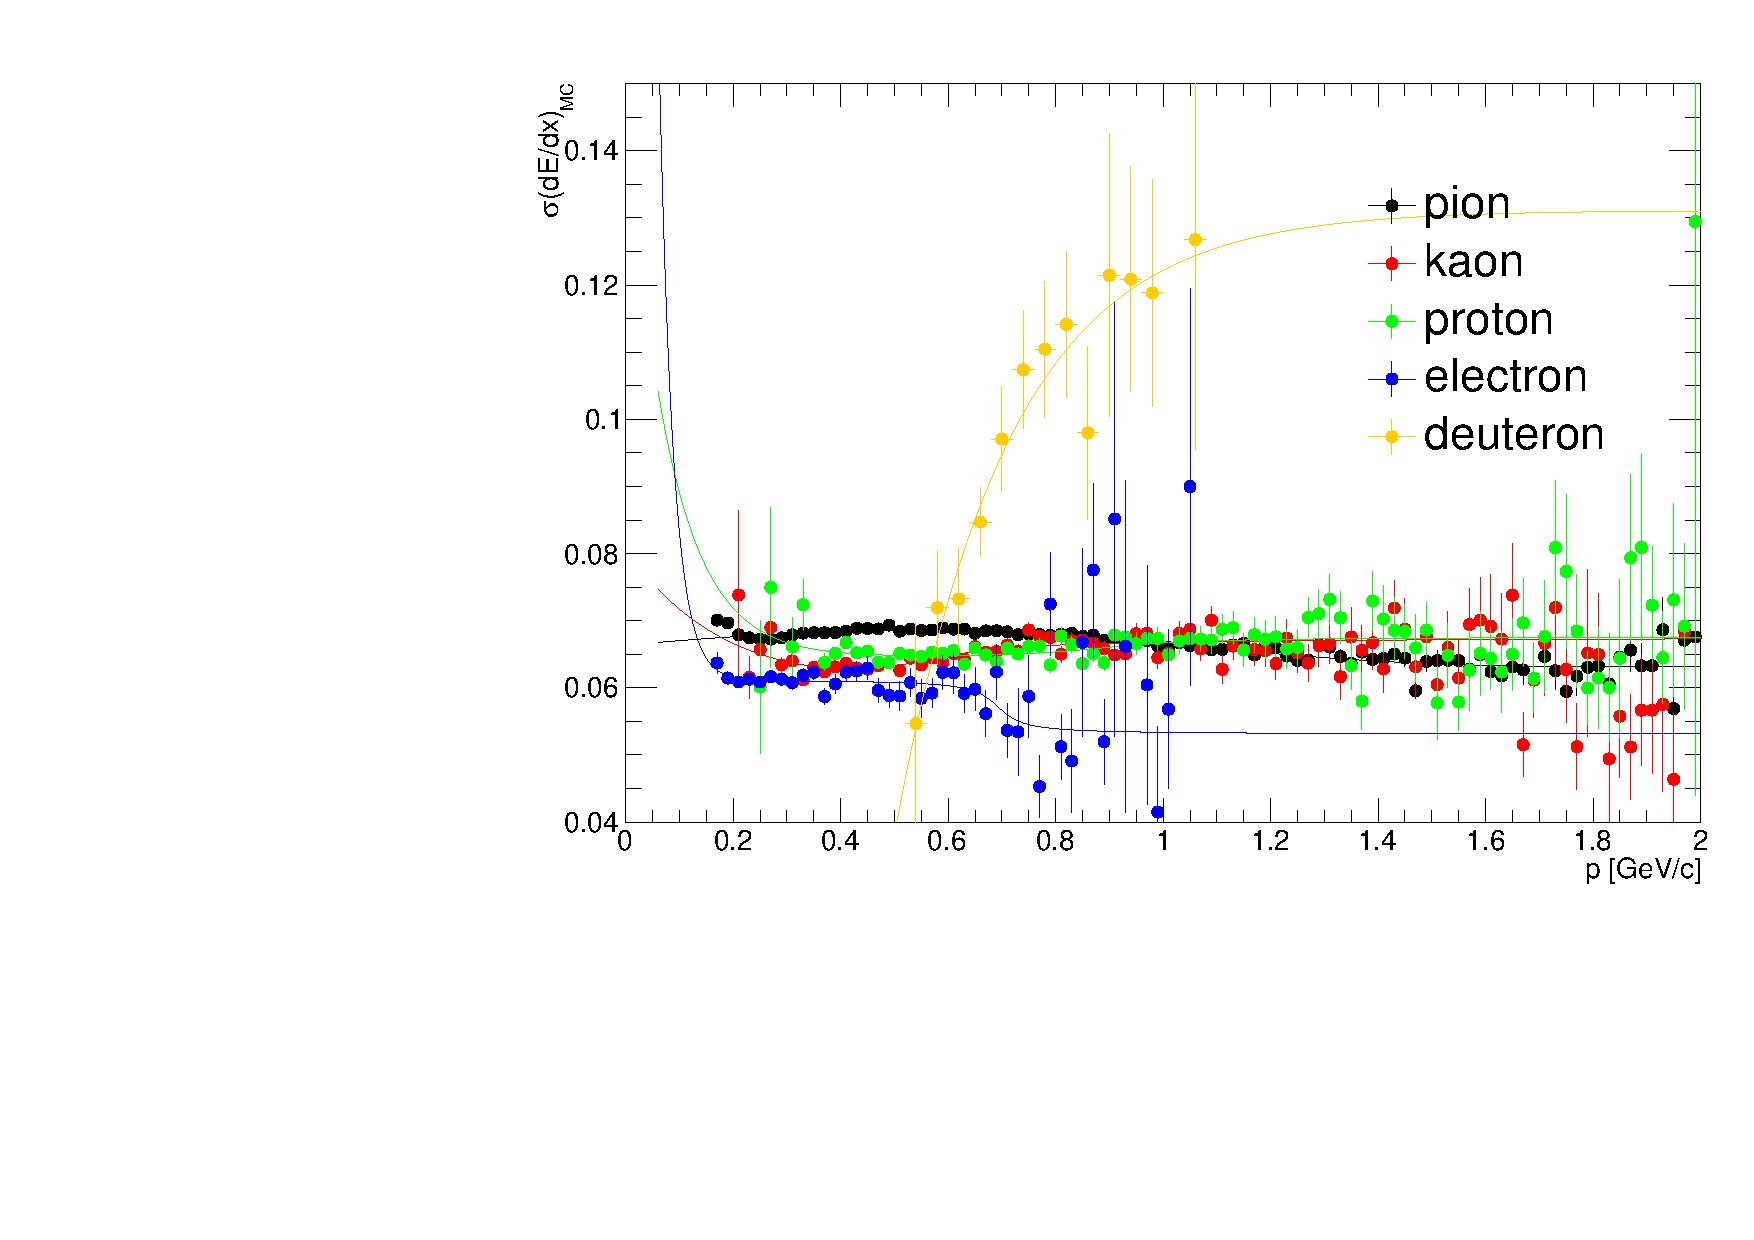
\includegraphics[width=\linewidth]{graphics/corrections/dEdxWidth_allPIDs.pdf}\vspace*{-10pt}}}
  \end{subfigure}\\
  \begin{subfigure}[b]{\linewidth}\addtocounter{subfigure}{1}{
                \subcaptionbox{\label{fig:dEdxWidthData}}{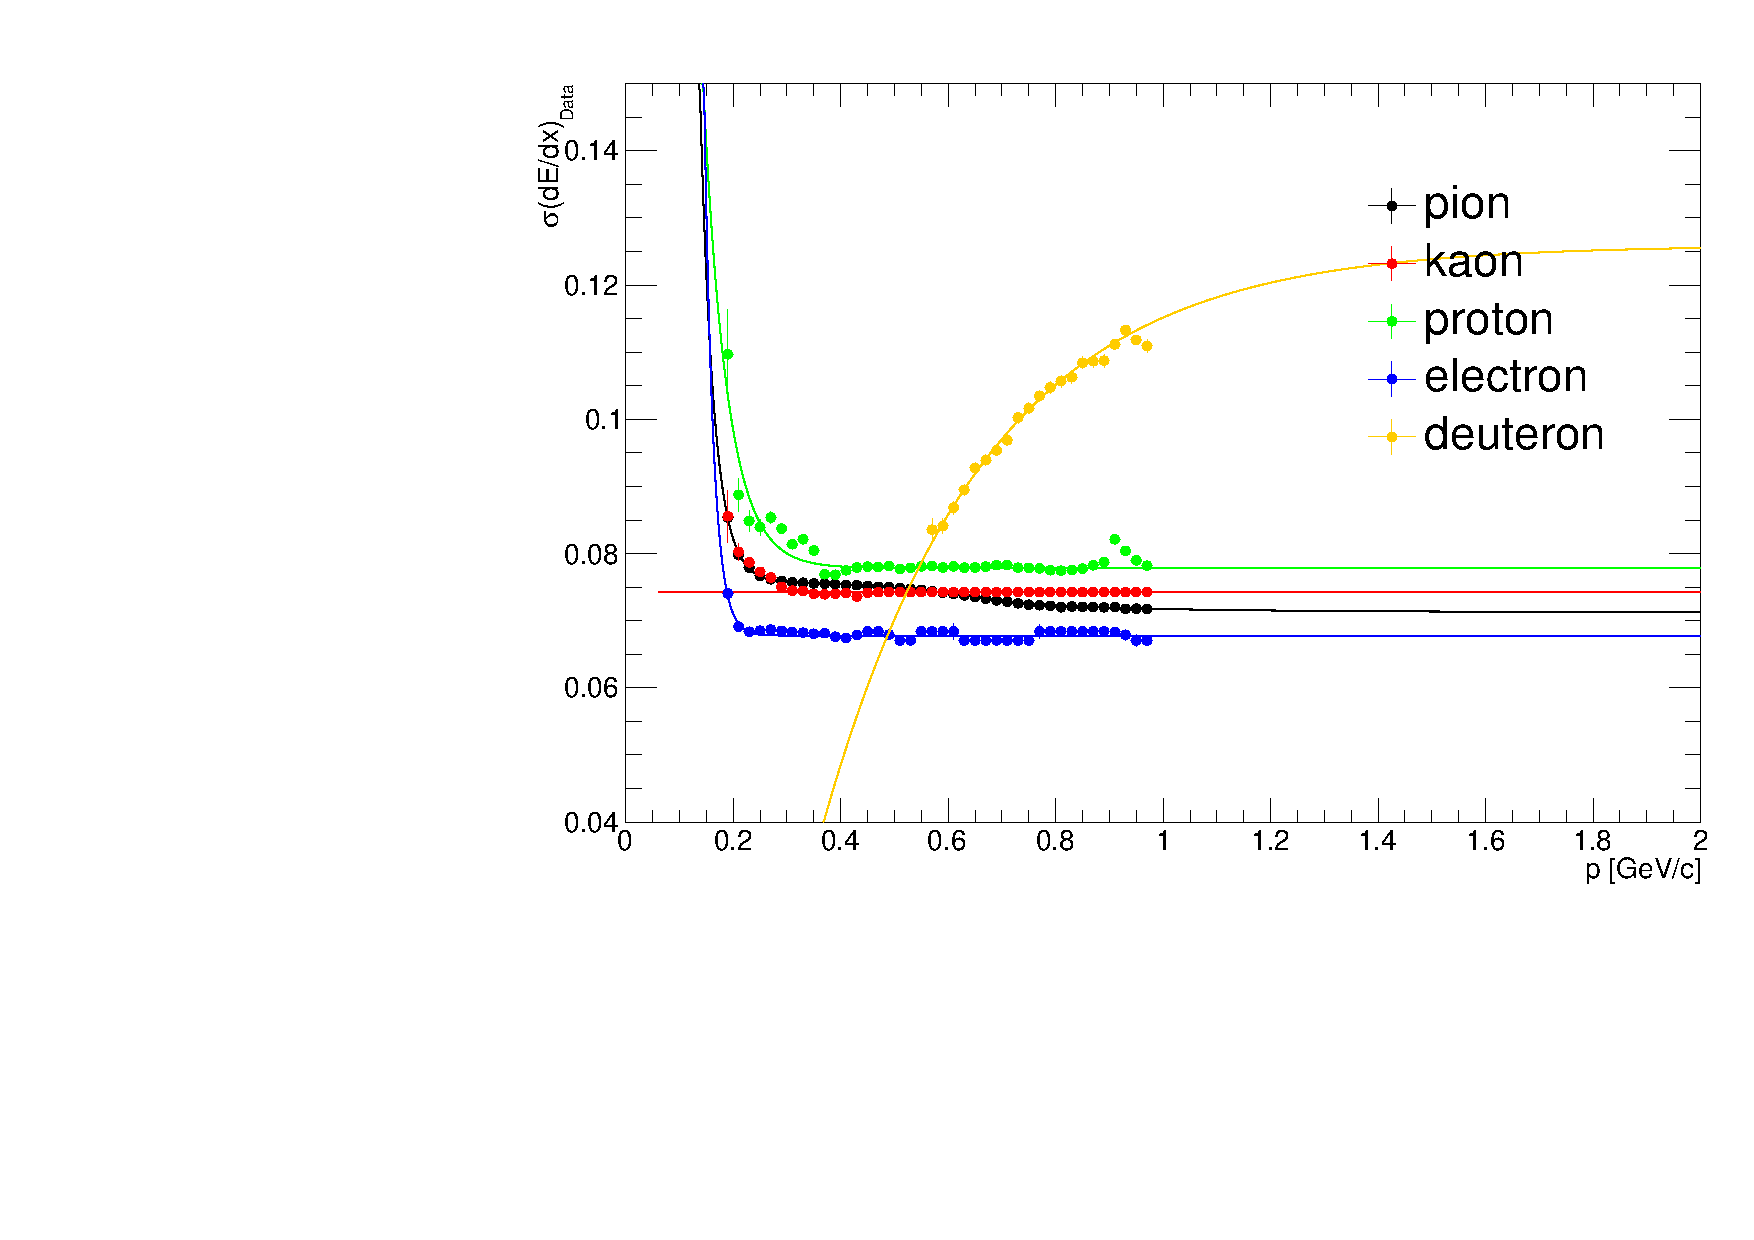
\includegraphics[width=\linewidth]{graphics/corrections/dEdxWidth_allPIDs_data.pdf}\vspace*{-10pt}}}
  \end{subfigure}
}%
\caption[Parameters of track dE/dx as a function of reconstructed momentum for a few particle species.]{Difference between MPV of dE/dx predicted by Bichsel parametrization and obtained from the fit of Eq.~\eqref{eq:expTail} to dE/dx distribution in the data (\ref{fig:dEdxMeanOffsetData}) and MC sample (\ref{fig:dEdxMeanOffsetMC}) and dE/dx width parameter in data (\ref{fig:dEdxWidthData}) and MC (\ref{fig:dEdxWidthMC}) as a function of reconstructed particle momentum for a few particle species. Solid lines represent fits to points of corresponding color.}\label{fig:dEdxParametersMC}
\end{figure}
%---------------------------


\begin{equation}\label{eq:dEdxParametrization}
	g(p) = P_{1} + P_{2}\cdot \exp{\left(-P_{3}\cdot p\right)} + P_{4}\cdot \arctan{\big(P_{5}\cdot(p-P_{6})\big)}
\end{equation}



\begin{table}[ht!]\centering
\subcaptionbox{\label{fig:vvv}}{
 \begin{tabular}{r||c|c|c|c|c|c||c|c|c|c|c|c}%\hline
 \multirow{2}{*}{\textbf{PID}} &  \multicolumn{6}{c||}{\bm{$\langle dE/dx\rangle_{\textrm{\textbf{Bichsel}}} - \langle dE/dx\rangle_{\textrm{\textbf{MC}}}$}} & \multicolumn{6}{c}{\bm{$\sigma(dE/dx)_{\textrm{\textbf{MC}}}$}} \\ \cline{2-13}
  & $P_{1}$ & $P_{2}$ & $P_{3}$ & $P_{4}$ & $P_{5}$ & $P_{6}$ & $P_{1}$ & $P_{2}$ & $P_{3}$ & $P_{4}$ & $P_{5}$ & $P_{6}$ \\ \Xhline{2\arrayrulewidth}
 $\bm{\pi^{\pm}}$ & \scriptsize3.293e-8 & \scriptsize2.237e-8 & \scriptsize4.399 & \scriptsize& \scriptsize& \scriptsize& \scriptsize0.0668 & \scriptsize1.186 & \scriptsize28.683 & \scriptsize-1.5e-3 & \scriptsize7.887 & \scriptsize1.028\\ \hline
 $\bm{K^{\pm}}$ & \scriptsize3.068e-9 & \scriptsize-8.190e-6 & \scriptsize7.089 & \scriptsize& \scriptsize& \scriptsize& \scriptsize0.0664 & \scriptsize0.323 & \scriptsize-10.438 & \scriptsize& \scriptsize& \scriptsize\\ \hline
 $\bm{p,\bar{p}}$ & \scriptsize-3.061e-8 & \scriptsize-1.061e-5 & \scriptsize4.08 & \scriptsize& \scriptsize& \scriptsize& \scriptsize0.0674 & \scriptsize0.103 & \scriptsize-5.952 & \scriptsize& \scriptsize& \scriptsize\\ \hline
 $\bm{e^{\pm}}$ & \scriptsize-1.483e-7 & \scriptsize3.710e-7 & \scriptsize5.639 & \scriptsize& \scriptsize& \scriptsize& \scriptsize0.0590 & \scriptsize-0.009 & \scriptsize-194.42 & \scriptsize-1.81e-3 & \scriptsize26.392 & \scriptsize0.607 \\ \hline
 $\bm{d,\bar{d}}$ & \scriptsize-2.474e-6 & \scriptsize0.385 & \scriptsize21.719 & \scriptsize5.165e-7 & \scriptsize29.642 & \scriptsize0.781 & \scriptsize0.131 & \scriptsize-0.999 & \scriptsize4.749 & \scriptsize& \scriptsize& \scriptsize%\hline
\end{tabular}
}
\subcaptionbox{\label{fig:aaa}}{
\begin{tabular}{r||c|c|c|c|c|c||c|c|c|c|c|c}%\hline
 \multirow{2}{*}{\textbf{PID}} &  \multicolumn{6}{c||}{\bm{$\langle dE/dx\rangle_{\textrm{\textbf{Bichsel}}} - \langle dE/dx\rangle_{\textrm{\textbf{Data}}}$}} & \multicolumn{6}{c}{\bm{$\sigma(dE/dx)_{\textrm{\textbf{Data}}}$}} \\ \cline{2-13}
  & $P_{1}$ & $P_{2}$ & $P_{3}$ & $P_{4}$ & $P_{5}$ & $P_{6}$ & $P_{1}$ & $P_{2}$ & $P_{3}$ & $P_{4}$ & $P_{5}$ & $P_{6}$ \\ \Xhline{2\arrayrulewidth}
 $\bm{\pi^{\pm}}$ & \scriptsize-1.236e-8 & \scriptsize1.777e-7 & \scriptsize-9.938 & \scriptsize& \scriptsize& \scriptsize& \scriptsize0.0738 & \scriptsize16.86 & \scriptsize39.44 & \hspace*{-3pt}\scriptsize-1.704e-3\hspace*{-2pt} & \scriptsize~6.482~ & \scriptsize0.628\\ \hline
 $\bm{K^{\pm}}$ & \scriptsize5.49e-10 & \scriptsize-2.732e-6 & \scriptsize-7.712 & \scriptsize& \scriptsize& \scriptsize& \scriptsize0.0743 & \hspace*{-2pt}\scriptsize2.67e-5\hspace*{-2pt} & \scriptsize7.17089 & \scriptsize& \scriptsize& \scriptsize\\ \hline
 $\bm{p,\bar{p}}$ & \scriptsize-2.140e-7 & \scriptsize0.0421 & \scriptsize48.305 & \scriptsize7.512e-8 & \scriptsize15.544 & \scriptsize0.575 & \scriptsize0.0779 & \scriptsize1.822 & \scriptsize22.4277 & \scriptsize& \scriptsize& \scriptsize\\ \hline
 $\bm{e^{\pm}}$ & \scriptsize6.701e-8 & \scriptsize3.304e-7 & \scriptsize-7.845 & \scriptsize& \scriptsize& \scriptsize& \scriptsize0.0678 & \scriptsize468.9 & \scriptsize59.4001 & \scriptsize& \scriptsize& \scriptsize\\ \hline
 $\bm{d,\bar{d}}$ & \scriptsize-1.631e-7 & \scriptsize0.0818 & \scriptsize-18.91 & \scriptsize& \scriptsize& \scriptsize& \scriptsize0.1259 & \scriptsize-0.288 & \scriptsize3.28733 & \scriptsize& \scriptsize& \scriptsize%\\ \hline
\end{tabular}
}\caption[Parameters of functions from Fig.~\ref{fig:dEdxParametersMC} describing track dE/dx as a function of reconstructed momentum for a few particle species (STARsim MC).]{Parameters of functions from Fig.~\ref{fig:dEdxParametersMC} describing track dE/dx as a function of reconstructed momentum for a few particle species. Units of parameters $P_{i}$ are such that if one provides momentum in Eq.~\eqref{eq:dEdxParametrization} in GeV/$c$ the resultant offset of dE/dx MPV with respect to Bichsel parametrization is in GeV/cm, and the resultant $\sigma$ parameter is unitless.}\label{tab:dEdxParametersMC}
\end{table}



















\subsection{RP track acceptance and reconstruction efficiency}\label{sec:rpAccAndEff}
\subsection{TPC track acceptance and reconstruction efficiency}\label{sec:tpcAccAndEff}
\subsection{TOF acceptance, reconstruction and track-matching efficiency}\label{sec:tofAccAndEff}
\subsection{TPC vertex reconstruction efficiency}\label{sec:tpcVxRecoEff}
\section{Particle energy loss}\label{sec:energyLoss}
\section{Background subtraction}\label{sec:bkgdSubtraction}
\section{Unfolding}\label{sec:unfolding}